\documentclass[a4paper,12pt]{article}
 \usepackage[italian]{babel} 
\usepackage{graphicx}
\usepackage{caption}
\usepackage{geometry}
\usepackage{enumitem}
\usepackage{fancyhdr}
\usepackage{svg-extract}
\usepackage{hyperref}
\geometry{a4paper, top=1.5cm, bottom=1.5cm, left=1.5cm, right=1.5cm, }
\setlength{\parindent}{0pt} %\setlength{\parskip}{0,25cm plus1mm minus1mm}
\graphicspath{ {/Users/nicola/Documents/GitHub/lifemanager/images/Latex/} } 
\lhead{
\includegraphics[width=5cm]{logounitn.jpg}}
\rhead{
\includegraphics[width=3cm]{logolifemanager.png}}
\setlist[itemize]{leftmargin=5.5mm}




%\fancyhead[L]{
\includegraphics[width=5cm]{logounitn.jpg}}
\renewcommand{\headrulewidth}{0pt}
\raggedbottom

%-----------------------------------------TITOLO
 \title{LifeManager}
 \author{
 Corso di Ingegneria del software\\ \\Luca Boschiero, Mauro Meneghello, Nicola Turniano
 }
 \begin{document} 
 \maketitle
 \thispagestyle{fancy}
 %-----------------------------------------INFORMAZIONI STUD
\hrule
\begin{table}[!h] 
\begin{tabular}{l l l}
Gruppo T10\\
Deliverable 2\\
 \\
Mauro Meneghello & 217564 & mauro.meneghello@studenti.unitn.it \\
Luca Boschiero & 217460 & luca.boschiero@studenti.unitn.it \\
Nicola Turniano  & 271457 & nicola.turniano@studenti.unitn.it \\
\end{tabular}
\end{table}
\hrule
\vspace{1cm}

 %-----------------------------------------SVOLGIMENTO


\section*{Analisi dei componenti}
Nel seguente capitolo analizzeremo i componenti interni che costituiranno il nostro sistema, andando a definire una prima architettura al software {\scshape LifeManager}, e le relazioni tra questi componenti. 

In particolare, un componente rappresenta un’entità autonoma all’interno di un sistema o sottosistema; esso ha una o più interfacce (fornite o richieste), e gli elementi al suo interno sono nascosti ed inaccessibili eccetto che attraverso i mezzi forniti dalle sue interfacce.


Il risultato di questa analisi costituirà i vari \textit{Component Diagrams }riportati nelle figure sottostanti; inoltre per ogni singolo componente sarà descritto lo scopo e le sue interfacce.

\begin{center}
  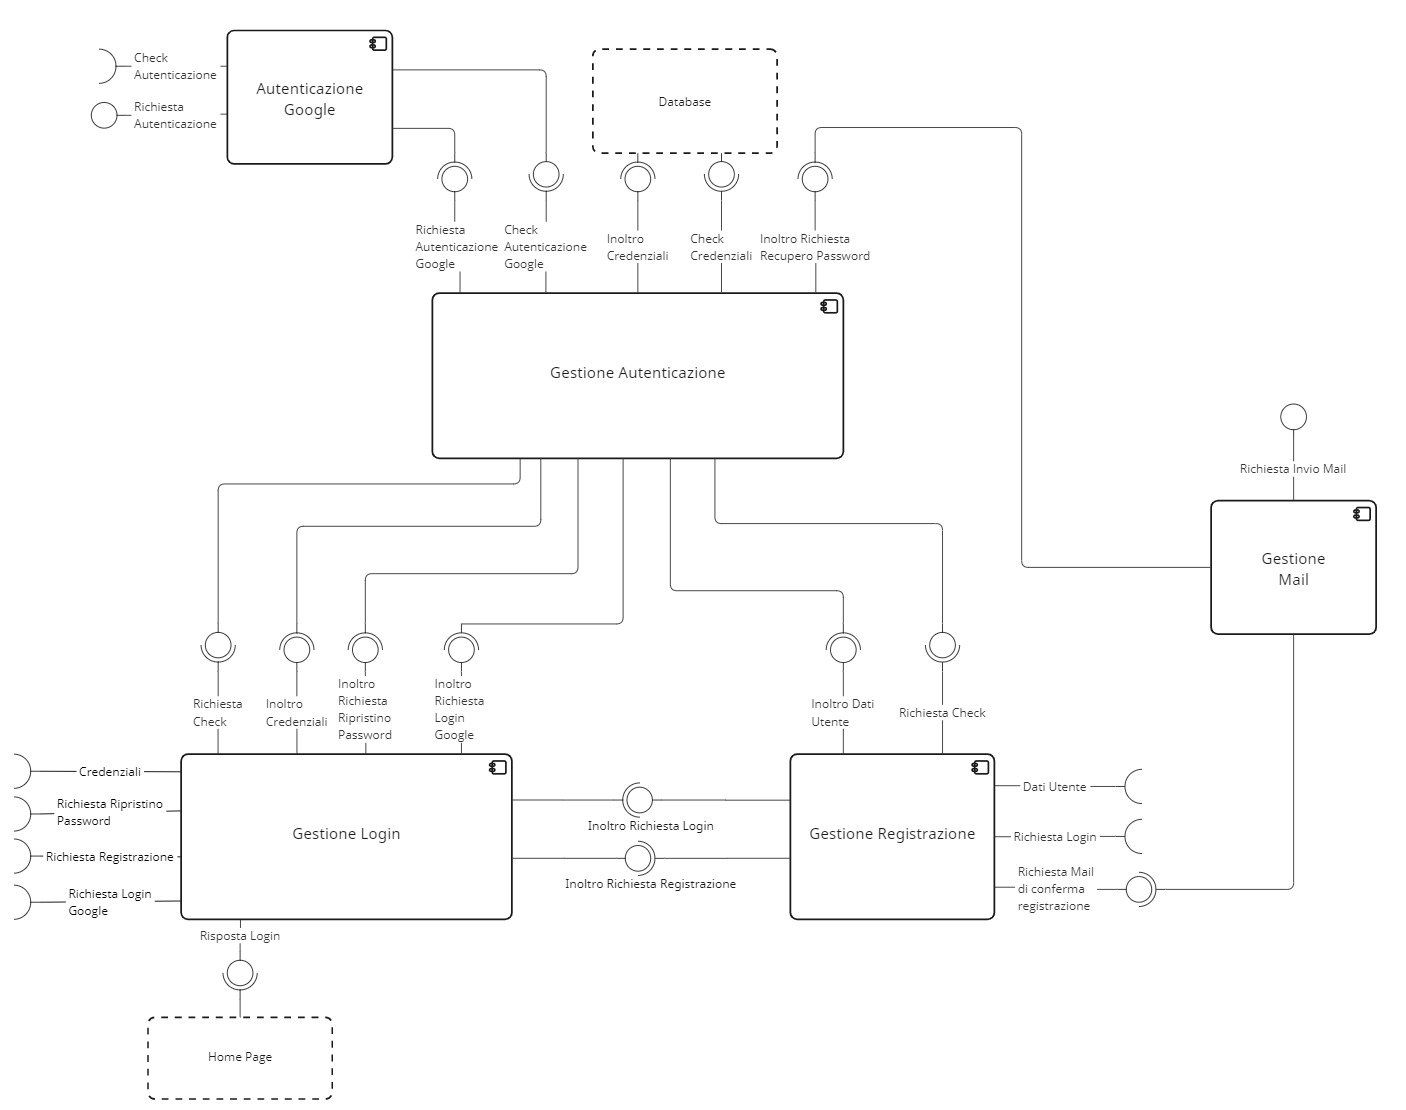
\includegraphics[width=15cm]{LoginRegistrazioneAutenticazione.jpg}
  \captionof{figure}{Component diagram Login, Registrazione, Autenticazione }
\end{center}

\subsection*{1 - Gestione Login}
\subsubsection*{Descrizione}
Questo componente permette di interfacciarsi direttamente con l’utente che desidera effettuare il login con le proprie credenziali. In particolare, verranno raccolti i dati dell’utente (credenziali) o eventuali richieste (recupero password) e inoltrati ad altri componenti interni per elaborarli.

\subsubsection*{Interfacce richieste}
\begin{itemize} \setlength\itemsep{0.01em}
\item {\sffamily Credenziali}: qualcosa.
\item {\sffamily Richiesta check}: qualcosa.
\item {\sffamily Richiesta ripristino password}: qualcosa.
\item {\sffamily Richiesta login Google}: qualcosa.
\item {\sffamily Richiesta registrazione}: qualcosa.
\item {\sffamily Richiesta login}: qualcosa.
\end{itemize}

\subsubsection*{Interfacce fornite}
\begin{itemize} \setlength\itemsep{0.01em}
\item {\sffamily Risposta login}: qualcosa.
\item {\sffamily Inoltro richiesta registrazione}: qualcosa.
\item {\sffamily Inoltro credenziali}: qualcosa.
\item {\sffamily Inoltro richiesta ripristino password}: qualcosa.
\item {\sffamily Inoltro richiesta login Google}: qualcosa.
\end{itemize}





\subsection*{2 - Gestione registrazione}
\subsubsection*{Descrizione}
Questo componente permette di interfacciarsi con l’utente per permettere la registrazione al sistema e la creazione di un nuovo account. I dati raccolti verranno smistati agli altri componenti che li elaboreranno.

\subsubsection*{Interfacce richieste}
\begin{itemize} \setlength\itemsep{0.01em}
\item {\sffamily Dati utente}: qualcosa.
\item {\sffamily Richiesta registrazione}: qualcosa.
\item {\sffamily Richiesta check}: qualcosa.
\item {\sffamily Richiesta mail}: qualcosa.
\end{itemize}

\subsubsection*{Interfacce fornite}
\begin{itemize} \setlength\itemsep{0.01em}
\item {\sffamily Richiesta mail conferma registrazione}: qualcosa.
\item {\sffamily Richiesta login}: qualcosa.
\item {\sffamily Inoltro dati utente}: qualcosa.
\item {\sffamily Scrittura database}: qualcosa.
\end{itemize}

\subsection*{3 - Gestione autenticazione}
\subsubsection*{Descrizione}
Questo componente è il responsabile della verifica dei dati inviati (dati di login o registrazione) e quindi dell’autenticazione degli utenti al sistema.
\subsubsection*{Interfacce richieste}
\begin{itemize} \setlength\itemsep{0.01em}
\item {\sffamily Inoltro dati utente}: qualcosa.
\item {\sffamily Inoltro credenziali}: qualcosa.
\item {\sffamily Richiesta ripristino password}: qualcosa.
\item {\sffamily Richiesta login Google}: qualcosa.
\item {\sffamily Check credenziali}: qualcosa.
\item {\sffamily Check autenticazione Google}: qualcosa.
\end{itemize}

\subsubsection*{Interfacce fornite}
\begin{itemize} \setlength\itemsep{0.01em}
\item {\sffamily Risposta check}: qualcosa.
\item {\sffamily Richiesta check}: qualcosa.
\item {\sffamily Inoltro richiesta ripristino password}: qualcosa.
\item {\sffamily Inoltro richiesta autenticazione Google}: qualcosa.
\item {\sffamily Inoltro credenziali}: qualcosa.

\end{itemize}

\subsection*{4 -  Autenticazione con Google}
\subsubsection*{Descrizione}
Qualcosa
\subsubsection*{Interfacce richieste}
\begin{itemize} \setlength\itemsep{0.01em}
\item {\sffamily titolo}: qualcosa.
\end{itemize}

\subsubsection*{Interfacce fornite}
\begin{itemize} \setlength\itemsep{0.01em}
\item {\sffamily titolo}: qualcosa.
\end{itemize}









%_{_{_{_{_{_{_{_{_{_{_{_{_{_{_{_{_{_{_{_{ALLA FINE_{_{_{_{}}}}}_{_{_{_{_{}}}}}}
\vspace{15cm}
\hrule
\vspace{0.5cm}


Mauro Meneghello - matricola 217564 - mauro.meneghello@studenti.unitn.it

Luca Boschiero - matricola 217460 -  luca.boschiero@studenti.unitn.it

Nicola Turniano - matricola 217457 - nicola.turniano@studenti.unitn.it

%-----------------------------------------
 \end{document}